
%(BEGIN_QUESTION)
% Copyright 2009, Tony R. Kuphaldt, released under the Creative Commons Attribution License (v 1.0)
% This means you may do almost anything with this work of mine, so long as you give me proper credit

Suppose the flow control valve in this three-element control system is slow to respond because it does not have a volume booster to help actuate it quickly:

$$\includegraphics[width=15.5cm]{i04344x01.eps}$$

Perform a ``thought experiment'' illustrating how this slow valve response compromises the feedforward control quality.  After that, explain how the proper addition of a lead/lag (I'll let you determine which!) function block could help address this problem.

\vskip 10pt

Next, explain how the judicious use of {\it cascade} control would be a better solution to the problem.

\vskip 20pt \vbox{\hrule \hbox{\strut \vrule{} {\bf Suggestions for Socratic discussion} \vrule} \hrule}

\begin{itemize}
\item{} Identify at least one {\it mechanical} solution to this problem.
\item{} Explain the significance of the ``+'' symbols next to the summer input lines.  How well would the system work if one or more of these inputs were inverting (``$-$'') rather than non-inverting?
\item{} Suppose the suction produced at the discharge line by the pumps proved to be a significant load in the system (i.e. starting or stopping pumps caused excursions in the vessel's level).  Explain how you might incorporate feedforward control to stabilize liquid level against that load.
\end{itemize}

\underbar{file i04344}
%(END_QUESTION)





%(BEGIN_ANSWER)


%(END_ANSWER)





%(BEGIN_NOTES)

A sluggish pneumatic valve has a {\it lag} characteristic.  In order to counter-act this lag behavior, we may add a {\it lead} function block to the signal path.

\vskip 10pt

It is probably best to add the lead function before the summing relay so that only the feedforward signal will be affected by it, and not the feedback controller:

$$\includegraphics[width=15.5cm]{i04344x02.eps}$$

\filbreak

A solution implementing cascade control would be best because it would address the problem at its source -- the sluggishness of the valve.  Placing a flow transmitter and a slave flow controller at the valve will make the valve respond more like it should for all conditions:

$$\includegraphics[width=15.5cm]{i04344x03.eps}$$

%INDEX% Control, strategies: feedforward with dynamic compensation (lead/lag)

%(END_NOTES)


